%%| filename: bayes_rule
%%| format: svg

\usetikzlibrary{positioning,arrows.meta}

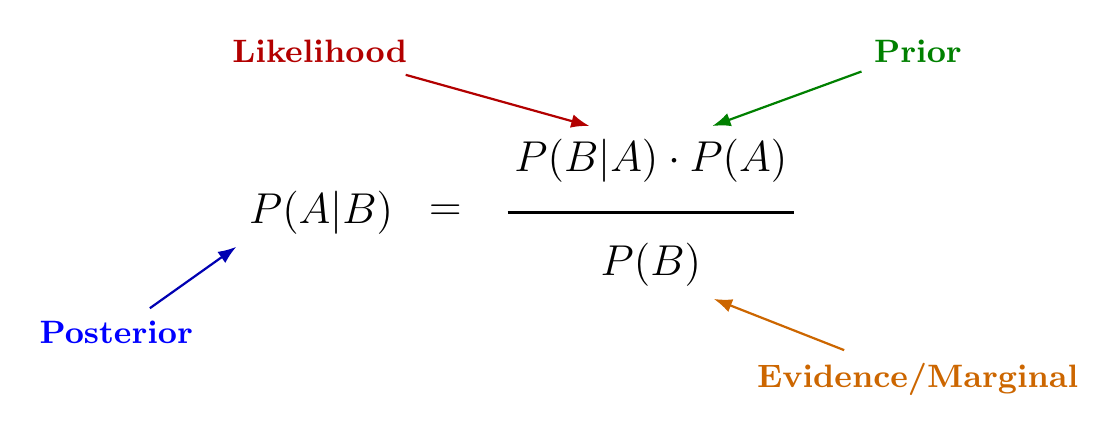
\begin{tikzpicture}[
  >=Latex,
  scale=1.3,
  transform shape,
  every node/.style={font=\large},
  label/.style={font=\small\bfseries},
  arrow/.style={->, thick}
]

% Fraction line first (as reference)
\node (frac_center) {};
\draw[thick] ([xshift=-1.4cm]frac_center.center) -- ([xshift=1.4cm]frac_center.center);

% Numerator (closer to line)
\node[above=0.05cm of frac_center] (numerator) {$P(B|A) \cdot P(A)$};

% Denominator (closer to line)
\node[below=0.05cm of frac_center] (evidence) {$P(B)$};

% Equals and posterior aligned with fraction line
\node[left=1.6cm of frac_center] (equals) {$=$};
\node[left=0.1cm of equals] (posterior) {$P(A|B)$};

% Labels with angled arrows and colors
\node[below left=0.6cm and 0.3cm of posterior, label, color=blue!70!blue] (post_label) {Posterior};
\draw[arrow, blue!70!black] (post_label) -- (posterior.south west);

\node[above left=0.5cm and 0.8cm of numerator, label, color=red!70!black] (lik_label) {Likelihood};
\draw[arrow, red!70!black] (lik_label) -- ([xshift=-0.6cm]numerator.north);

\node[above right=0.5cm and 0.6cm of numerator, label, color=green!50!black] (prior_label) {Prior};
\draw[arrow, green!50!black] (prior_label) -- ([xshift=0.6cm]numerator.north);

\node[below right=0.5cm and 0.3cm of evidence, label, color=orange!80!black] (ev_label) {Evidence/Marginal};
\draw[arrow, orange!80!black] (ev_label) -- (evidence.south east);

\end{tikzpicture}
